\documentclass[a4j,11pt]{jreport}
\usepackage[dvips]{graphicx}
\usepackage{subfigure}
\usepackage{epsfig}
\usepackage{ascmac} %framebox
\usepackage{ulinej}%行替え可能な下線
\usepackage{title1}
\usepackage{array, booktabs, float}
\usepackage{amsmath}
%-----
\newcommand{\epsfile}{\epsfig}
\renewcommand{\sl}{}
\renewcommand{\em}{}
\renewcommand{\bibname}{参考文献}
%-----
%\title{}%ここは空にしておく
\newcommand{\SKTitleYear}{令和6年度}
\newcommand{\SKTitleSemester}{秋学期}
\newcommand{\SKTitleClass}{卒業研究3 (BI)}
\newcommand{\SKTitleTeacher}{上山憲昭} %指導教員の氏名を記入
\newcommand{\SKTitleTeacherClass}{教授}
\newcommand{\SKTitleUniv}{立命館大学}
\newcommand{\SKTitleUnivDepart}{情報理工学部}
\newcommand{\SKTitleDepartment}{セキュリティ・ネットワークコース}
\newcommand{\SKTitleSort}{学士論文}
\author{羽田秀平}
\newcommand{\SKTitleTitle}{\ulinej{
タイムスタンプを用いた公平なオンラインチケット販売方式
}}
\newcommand{\SKTitleID}{26002103035}
\newcommand{\SKdate}{令和6年1月31日}
%-----
\setlength{\oddsidemargin}{10mm} %文書左位置設定(※タイトルがずれる)
%-----
\begin{document}
\maketitle
\chapterA{概要}
先着順でオンラインチケットを販売するオンラインチケット販売サイトでは,
販売サーバに購入要求が到着した順番で,チケットを販売するユーザを選択している.
しかし,公平性という観点では,購入要求のパケットをネットワークに送出した時刻が
早い順番で購入者を選択することが望ましい.
そのため販売サーバから遠い場所にいるユーザや,高負荷のネットワークを経由したユーザは,
購入要求パケットの送出時刻が早くても,
チケットを購入できない可能性がある.とくに大量のボットを用いて自動でチケットを
購入するユーザが存在する場合,このような問題はより顕著となる.

本稿ではこのような公平性の問題を解決するために,
チケット購入の要求パケットを受信したルータが受信時刻をパケットの
ヘッダ内に記述し,販売サーバはパケットに記述された受信時刻の早い順番でチケット購入者を選択することを提案する.
そしてP4 (Programming Protocol-independent Packet Processors)スイッチ[1]を
用いて,タイムスタンプ(TS)機能を実装し,処理遅延に関する評価結果を示す.

\tableofcontents

\chapter{序論}
\section{研究の背景}
コロナ禍以降,オンライン販売サイトでのチケット販売が増加している.
販売方法として抽選販売と先着販売があり,
大規模なライブやイベントのチケット販売では抽選販売が主流である.
これは,抽選販売では集客数が十分に確保されることが予想されており,
購入者をランダムに選択することで公平性を担保することができるためである.
また先着販売は,小中規模のライブやイベントで用いられることが多く,
これは大規模なライブやイベントと異なり,集客が不安定であることや,
先着順で販売することによって顧客の購買欲を高める目的があると考えられる.
二つの販売システムを比較すると,先着販売では一部地域でネットワークの遅延が発生すると,
ユーザがチケット販売サーバに対して送信された購入要求のパケットが,
遅延が無かった本来の時刻で到着しない可能性がある.
先着販売は,パケットがチケット販売サーバで処理された順番によって,
チケットの購入が確定することから,先着販売では公平性が確保されない可能性がある.
また販売サーバから距離が離れているユーザは,
近い距離にいるユーザと同時刻に購入要求のパケットを送出しても,
到着時刻が遅れる可能性がある.
これらの問題に対して,一部のユーザが不正なボットを用いて,
販売サーバに対して不正なアクセスを繰り返すことによって,
チケットの購入を試みた場合,販売サーバへの負荷が増すだけでなく,
ネットワークの遅延も発生し,
問題は更に深刻になると考えられる.


\section{研究の目的}
このような公平性の問題を解決するために本稿では新たな提案方式として,
ユーザが送出したチケット購入要求のパケットが,
チケット販売サーバに到着するまでに通過するルータで受信された場合、
その受信時刻をパケットのヘッダー部分に記録する仕組みを導入することによって解決する.
この処理はユーザがパケットを送出した地点からできるだけ近いノードであることが望ましい.
これにより送信時刻とパケットのヘッダーに記録される時刻の乖離が減少するので,
チケット販売サーバが,このパケットのヘッダに記録された時刻を参照し,
購入処理を行うことによって公平性を確保することが可能である.
この提案方式を実現することによってチケット販売サーバから距離が離れたユーザや,
パケットがチケット販売サーバに到着するまでの途中経路のネットワーク内で輻輳が発生していた場合でも,公平性が確保される.

提案方式を実現するにあたって,
本稿ではP4スイッチにパケットに対してTS付与機能を実装し,
各ノードに配置することで,問題を解決することを目指す.
また,提案方式の有効性を評価するために,
TS付与条件の比較処理及びTS付与処理の時間を測定し,
送信のみを行う場合と比較することによって提案方式の有効性を評価する.
最後に,提案方式の改善として,TS付与処理を行うルータを最適に配置する問題を定式化することで最適配置問題を解決することを目指す.

\chapter{関連研究}

\section{タイムスタンプ}
タイムスタンプに焦点を当てた研究として,\cite{P4STA}がある.
\cite{P4STA}では従来のネットワーク制御および管理アプリケーションのQoS要件には,
スイッチ,ルータ,仮想ネットワーク機能(VNF)などの
ネットワーク要素の正確な測定を実行する機能が必要性について述べている.
この要求を満たすために,転送遅延が1µs以下で数百ギガビット/秒の広帯域幅を提供する最新のネットワークスイッチを利用した場合,
測定機器に高い時間精度と損失検出要件が課せられるが,既存のソフトウェアベースの測定ツールでは満たされないことを研究背景として述べている.
この問題に対して,ソフトウェアベースのトラフィック負荷生成の柔軟性とハードウェアパケットタイムスタンプの精度を組み合わせた,
オープンソースフレームワークであるP4STAを提案手法として紹介している.
市販のP4スイッチを使用して得られた評価結果では,
これらのプログラマブルデータプレーンプラットフォームで,
最大1nsの時間分解能を実現できたことが示しており,P4-SmartNICとFPGAでの実験においても同様の結果が得られたことが述べられている.
そして,複数のソフトウェアベースの負荷ジェネレータのトラフィック負荷を組み合わせて,
ポートあたり最大100Gbit/sの測定負荷を実現する方法を示している.

\section{P4スイッチが導入された株式市場のネットワーク}
P4スイッチが高機能性に着目し,実際のネットワークに導入された研究として,\cite{LOBIN}がある.
\cite{LOBIN}では株式市場のアルゴリズム取引の発展を機械学習を用いて推進しているが,
機械学習を含めた計算処理に高速な実行速度が求められていることを述べている.
この株式市場における取引の遅延を短縮するにあたって,
機械学習の推論をプログラマブルネットワークデバイスにオフロードする,
つまりネットワーク内機械学習を行うことによって解決することを提案している.
この提案手法を実現するために,
高頻度の市場データフィードを使用して機械学習ベースの市場予測を提供するLOBINを紹介している.
この市場予測システムはLOBINで指値注文帳を作成し,プログラマブル スイッチ内で推論を実行することで実現している.
LOBINの性能を評価するために,NASDAQ’s Historical TotalView-ITCH sample dataを使用し,精度,遅延及びスループットを評価している.

\section{P4スイッチ間の時刻同期}
\cite{Clock Synchronization}では,P4スイッチ間の時刻同期について述べられている.
ネットワーク技術の進化によるインバンド ネットワーク テレメトリ (INT) の使用に関する継続的なテストでは、ネットワーク ノードのクロックの正確な時間同期の有用性と関連性が強調されているが,
INT機能では,大容量リンク(100 Gbps)でも各パケットにタイムスタンプをタグ付けできるため,参加ノード間の時間はマイクロ秒またはナノ秒のオーダーで高精度に同期する必要がある.
この文書ではINTの概要を示し、時刻同期の基本的な概念とコンポーネントを紹介し、次にP4スイッチにおけるハードウェア要素の現在の機能のレビューを含め、INT の場合の使用法を示している.

\chapter{提案方式}

\section{概要と特徴}

従来のオンラインチケット販売では,ユーザはチケットを購
入する際,ペイロードに購入情報が格納されたパケットをチケッ
ト販売サーバに送信し,チケット販売サーバで処理が完了した
タイミングで,ユーザのチケット購入が確定する.図 1 に,提案
する公平なオンラインチケット販売方式を示す.提案方式でも,
ユーザが送信したチケット購入の要求パケットが送信され,ネッ
トワーク内を経由してチケット販売サーバに到達する.ただし
提案方式では,ネットワーク内のノード (ルータ) において要求
パケットに対して TS 付与処理を実行する.できるだけユーザ
が要求パケットを送信してからの経過時間が短いタイミングで
TS をパケットに付与することが求められ,ユーザ端末からでき
るだけ近いノードであることが望ましい.チケット販売サーバ
は,要求パケットに付与された TS の値が小さい (早い) 順に,
チケット購入者を決定する.

\begin{figure}[htbp]
  \centering
  \includegraphics[width=1.0\linewidth]{data/soturon_teianshuhou.eps}
  \vspace{0mm}
  \caption{TSを用いた公平なオンラインチケット販売方式}
  \label{fig:teianshuhou}
\end{figure}

\section{パケットのIPアドレスを,サーバリストと一致するかの判定}
提案方式では,TS付与処理を行うルータが,
パケットの宛先アドレスがチケット販売サーバのアドレスであるかを判定する.
これにより,TS付与処理を行うべきパケットを特定することができる.
この判定処理はノード内で保存されたルーティングテーブルとIPアドレスをを比較することで実現する.

\section{TS付与}
TS付与処理は,BMv2を使用したP4スイッチで標準機能として備わってる,
時刻が逐次代入されるingress\_global\_timestampという変数,
から値を得ることによって時刻を得る.そしてパケットのヘッダのオプションフィールドに,
TSを付与することによって実現する.またTS付与処理は,
宛先アドレスがチケット販売サーバのアドレスであるパケット
に対してのみ実行する.

\section{チェックサムの更新}
チェックサムの更新は,TS付与処理を行った後のパケットのヘッダに対して,更新を行う.
この処理は,Egress Match-Action後にそれぞれのヘッダのオプションから値を参照し,チェックサムを更新することで実現する.


\section{時刻同期}
時刻同期は,TS付与処理を行うノードが,正確な時刻を取得し,TS付与処理を行うために必要である.
今回の提案方式では,P4スイッチからローカルPCの時刻を取得することによって,全てのP4スイッチの時刻が同期される.


\chapter{P4スイッチによる提案方式の実装}

\section{P4の概要と動作}

P4はネットワーク機器において,
パケットに含まれるデータに対してどのような処理を行うべきかを判断し実行処理を担うデータプレーンを
プログラムすることが可能な言語である.
従来のネットワークを制御をソフトウェアで行う技術,つまりSDN
(Software Defined Networking)では
Openflowが広く普及している.OpenflowはSDNを実現するプロトコルであり,
ネットワークにおいて複数存在するハードウェアの機能を1つの制御装置を用いて
制御することが可能である.
しかし,Openflowが扱うことができるパケットのヘッダフィールドは発展するとともに数が増え,
開発者にとって複雑性が増すばかりである.
P4はOpenflowとは異なり,ユーザが自由にパケットのヘッダフィールドを定義できる.
またスイッチのハードウェア実装を考慮せず実装することを可能にするAPIを提供することで抽象性を高めている.
以下がP4の特徴である.

\begin{quote}
  \begin{itemize}
    \item パケットのヘッダを自由に定義できる
    \item ターゲットデバイスに依存しない
  \end{itemize}
\end{quote}

\subsection{V1ModelでのP4の動作}
V1ModelはP4のアーキテクチャの一つであり,BMv2 simple switchで用いられいるアーキテクチャである.
このアーキテクチャの概要図を図\ref{fig:v1model}に示す.
このアーキテクチャではParser,Ingress Match Action,Egress Match Action及びDeparser
をP4によって記述し,プログラムを実行することができる.

\begin{figure}[htbp]
  \centering
  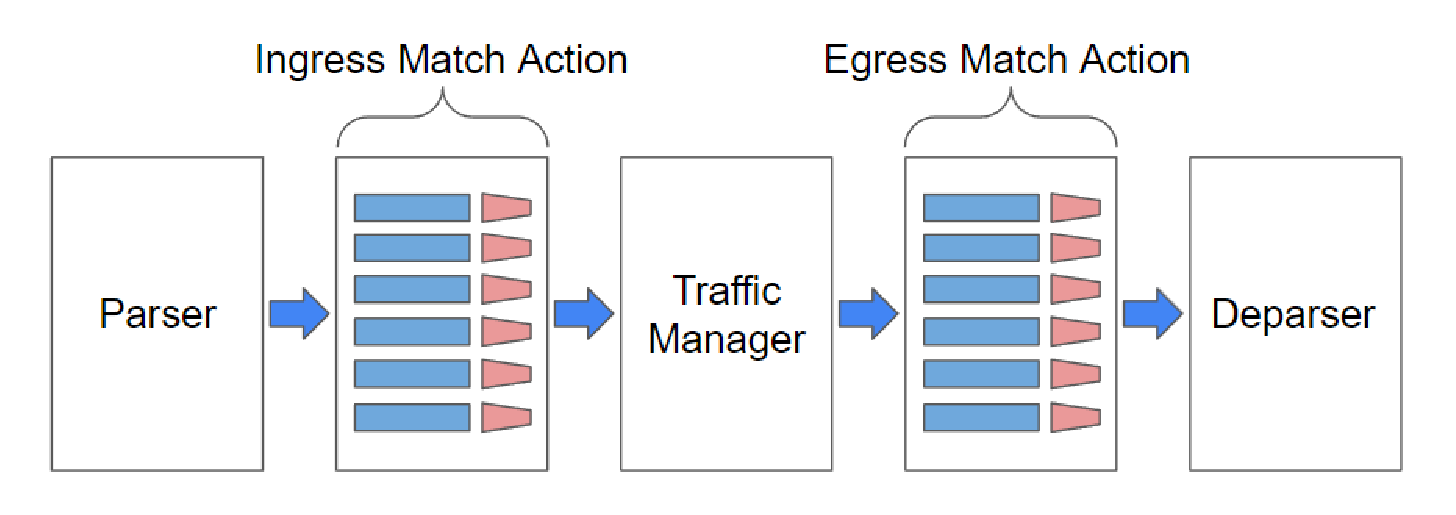
\includegraphics[scale=0.61]{data/v1model.eps}
  \vspace{0mm}
  \caption{V1modelアーキテクチャの概要図}
  \label{fig:v1model}
\end{figure}

\subsection{Parser}
Parserでは,パケットのフォーマットを解析して、さまざまなヘッダとメタデータを抽出する.
抽出したヘッダとメタデータは開発者が記述した状態遷移図に基づいて抽出される.
全ての状態遷移図はstart状態から始まり,到達したパケットと開発者が記述した状態遷移図の条件と照合し,
結果の真偽を通して,最終的にaccept状態もしくはreject状態に到達する.
accept状態に到達した場合,パケットは受け入れられ,処理を引き継ぐための情報を渡される.
またreject状態に到達した場合,パケットは破棄される.
Parserで抽出されたヘッダとメタデータは,Checksum Verificationによってチェックサムの検証が行われる.

\subsection{Ingress Match-Action}
Ingress Match-Actionでは,Parserで抽出したヘッダのフィールド値やメタデータを用いて,ヘッダに対してどのような処理を行うかを決定する.
行うことができる処理として,ヘッダのフィールド値を変更するだけでなく,
パケットのフィールド値を参照し,条件が一致すれば宛先アドレスや
ヘッダのフィールド値を変更及びパケットの複製・破棄を行うことができる.
フィールド値と条件との比較は,P4プログラムを制御するためのコントロールプレーンに保存されているテーブルを参照することで行われる.
このテーブルに値を送信する場合はP4runtimeなどのAPIを用いて送信する.

\subsection{Traffic Manager}
Traffic Managerでは,パケットのキューイング処理やレプリケーション処理とそのスケジューリングを行う.

\subsection{Egress Match-Action}
Egress Match-Actionでは,Ingress Match-Actionと同じようにパケットのヘッダのフィールド値やメタデータを変更することができる.
Egress Match-Actionが存在するメリットの一つとして,Ingress Match-Actionで複製されたパケットをさらに処理することができるなど多くのメリットが存在する.
Egress Match-Actionで処理されたパケットのヘッダとメタデータは,Checksum updateによってチェックサムの修正が行われる.

\subsection{Deparser}
Deparserでは,これまでの処理で変更されたヘッダを再度パケットに結合する処理を行う.


\section{パケットヘッダのフォーマット}
P4スイッチTS付与処理行った場合のパケットへッダのフォーマットとWiresharkを用いて観測したTS処理後のパケットを図\ref{fig:packet_format}及び図\ref{fig:wireshark}に示す.
TimestampヘッダはIPパケットのOption部の位置に設けており,フィールド値にはUNIX時刻が格納されている.

\begin{figure}[htbp]
  \centering
  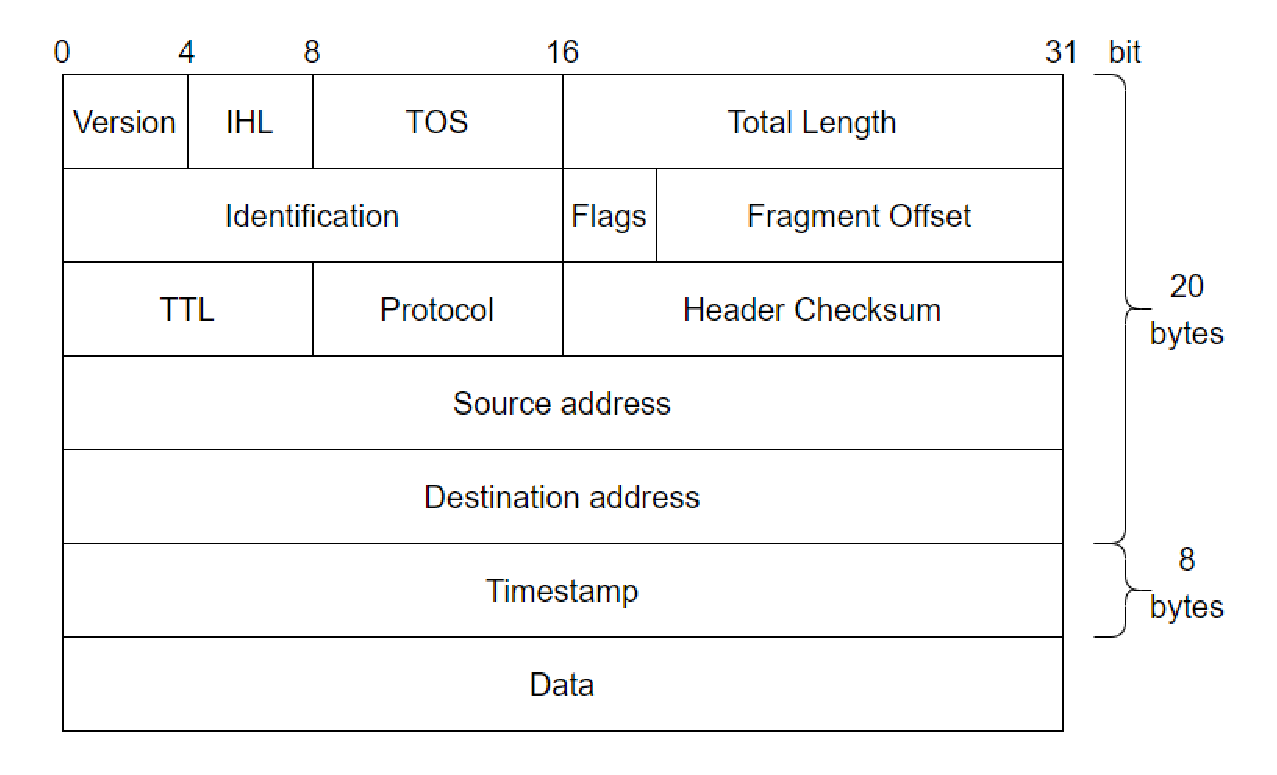
\includegraphics[scale=0.65]{data/packet_format.eps}
  \vspace{0mm}
  \caption{TS処理後のパケットフォーマット}
  \label{fig:packet_format}
\end{figure}

\begin{figure}[htbp]
  \centering
  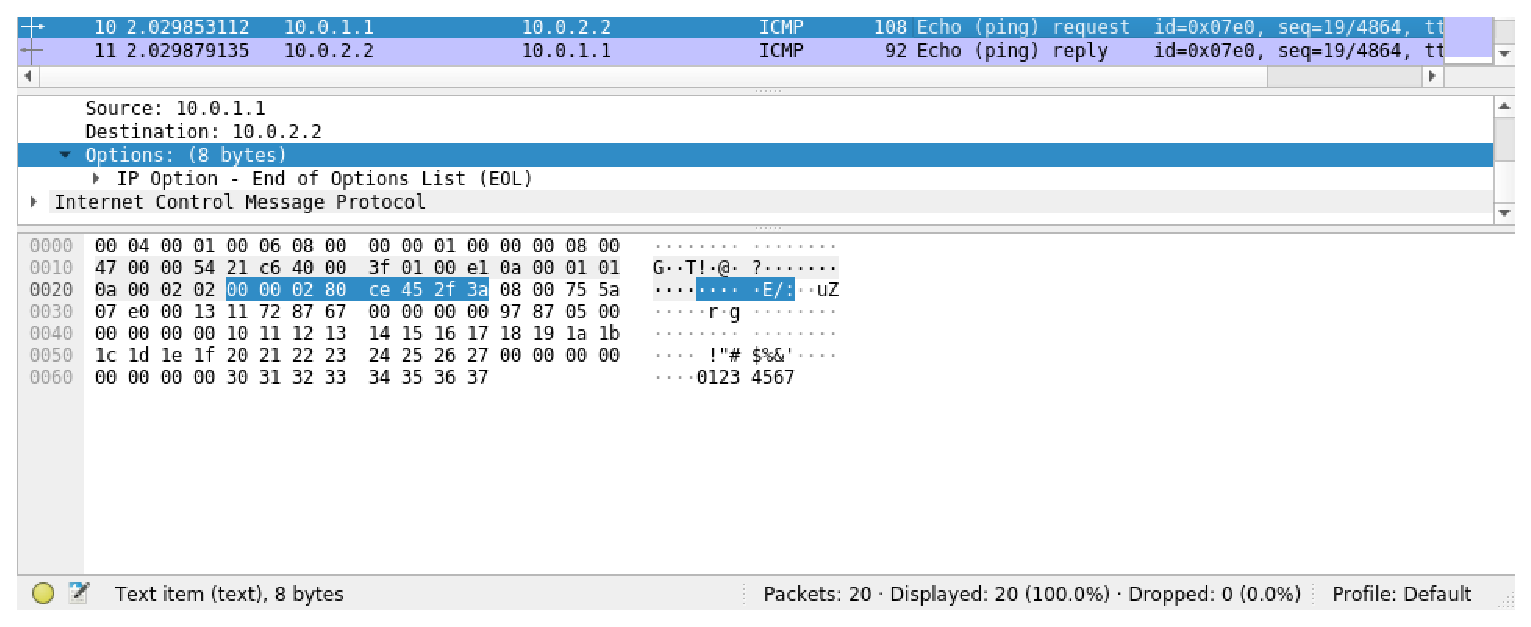
\includegraphics[scale=0.55]{data/wireshark3.eps}
  \vspace{0mm}
  \caption{Wiresharkを用いて観測したTS処理後のパケット}
  \label{fig:wireshark}
\end{figure}


\chapter{性能評価}

提案方式の有効性をソフトウェアベースの P4 スイッチを用
いた実装により評価する.性能評価に用いるモデルを図 2 に示
す.このモデルは VirtualBox 上で Ubuntu 20.04.6 LTS を使
用し,提案方式のプログラムはオープンソースのソフトウェアス
イッチである bmv2 の v1model アーキテクチャを使用して実装
した.動作させたモデルにおいて,クライアントが送出したパ
ケットは三つのルータを経由し,宛先であるチケット販売サー
バに到着する.この過程において,提案方式における付与条件
の比較及び TS 付与処理を,クライアントから 2 ホップ目にあ
たるルータにパケットが到着した際に実行した.この処理を行
うルータ以外は全てパケットの転送処理のみ行う.

\begin{figure}[htbp]
  \centering
  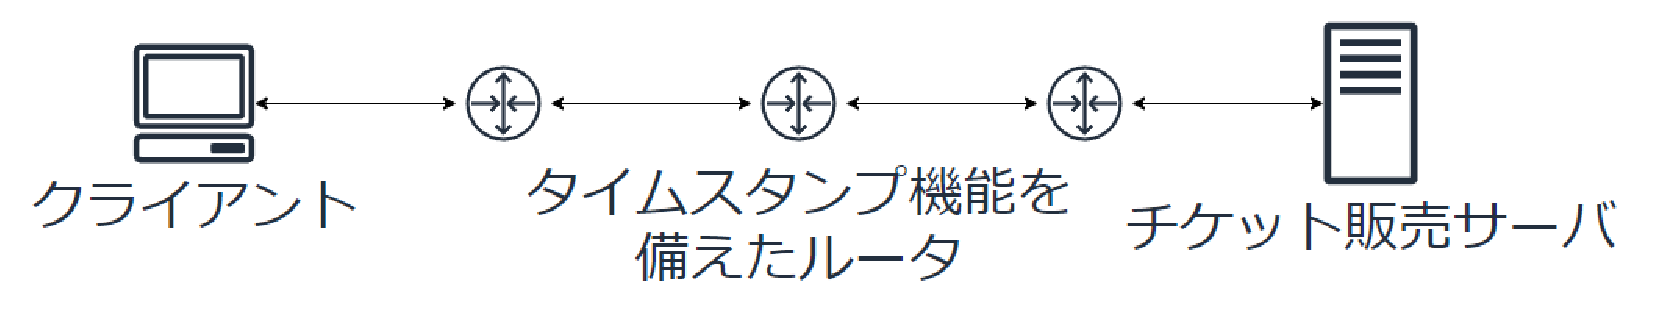
\includegraphics[scale=0.5]{data/soturon_network_koseizu2.eps}
  \vspace{0mm}
  \caption{性能評価モデル}
  \label{fig:seinouhyouka_model}
\end{figure}

\section{評価条件}
ユーザがチケット販売サーバを宛先としてパケットを送信し,
TS付与対象のパケットの識別処理とTS付与処理をルータで実
行した場合と,これらの処理を行わないでパケット送信処理のみ
実行した場合を100回ずつ試行し,各々の処理時間を測定した.
処理時間には,TS付与条件の比較処理及びTS付与処理,パケット送信処理の時間が
含まれている.

\section{性能評価}
図\ref{fig:shori}において提案方式TS付与処理を行なった
場合と,行わなかった場合の処理時間の差はマイクロ秒以下であ
ることが確認できる.例えばNTP(Network Time Protocol)
の時刻精度とは数ミリ秒から数百ミリ秒であり,提案方式の処
理時間は極めて小さいことが確認できる.

\begin{figure}[htbp]
  \centering
  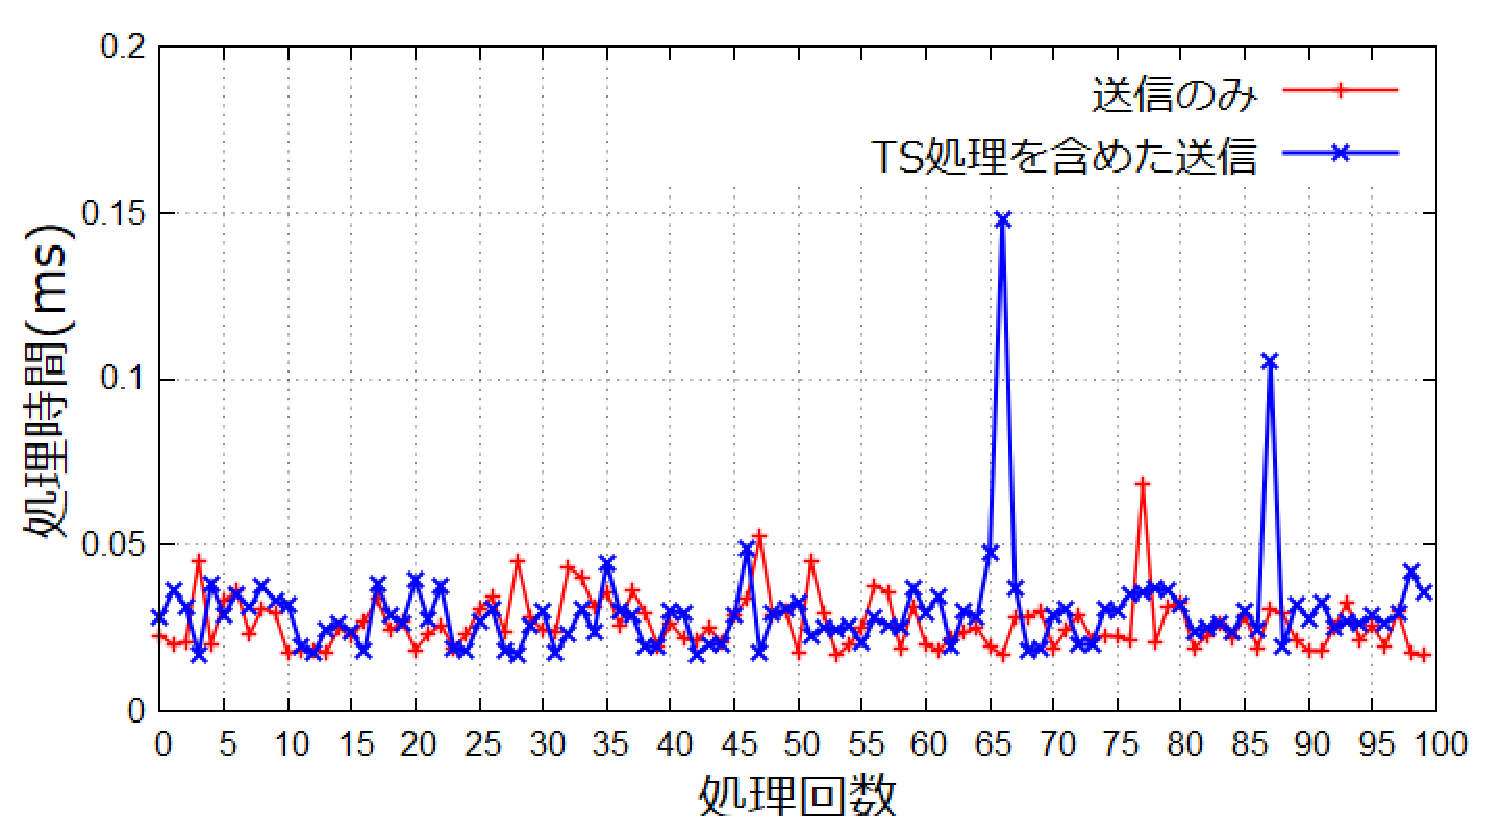
\includegraphics[scale=0.5]{data/soturon_shori_hikaku6.eps}
  \vspace{0mm}
  \caption{パケット処理時間の比較}
  \label{fig:shori}
\end{figure}

\chapter{提案方式の改善}

\section{P4スイッチの最適配置問題}
提案方式では,TS付与処理を行うルータをクライアントからできるだけ近いノードであり,全てのパケットがTS付与処理を行うルータを通過することが望ましいが,
P4スイッチが高額であるため,ネットワークのトポロジによっては,全てのルータにTS付与処理を行うことが難しい.
従って,TS付与処理を行うルータを最適に配置することが重要である.
性能評価より,TS付与処理の処理時間はマイクロ秒以下であるため,この処理時間を考慮する必要が無いことから,
通信速度を保ちつつ,TS付与処理を行うルータを最適に配置するには,ユーザとP4スイッチの距離ができるだけ近い距離であることと
運用されているISPのネットワークのトポロジのどのノードに配置することによって全てのパケットが通過するか考慮する必要がある.
よって,TS付与処理を行うルータの最適配置問題はこれらの条件を最小化することによって定式化できる.\\
\indent
この式を作成するにあたって,以下のISPのネットワークのトポロジを用いて,TS付与処理を行うルータの最適配置問題を解く.\\
以下の図はISPのネットワークのトポロジである.

\begin{figure}[htbp]
  \centering
  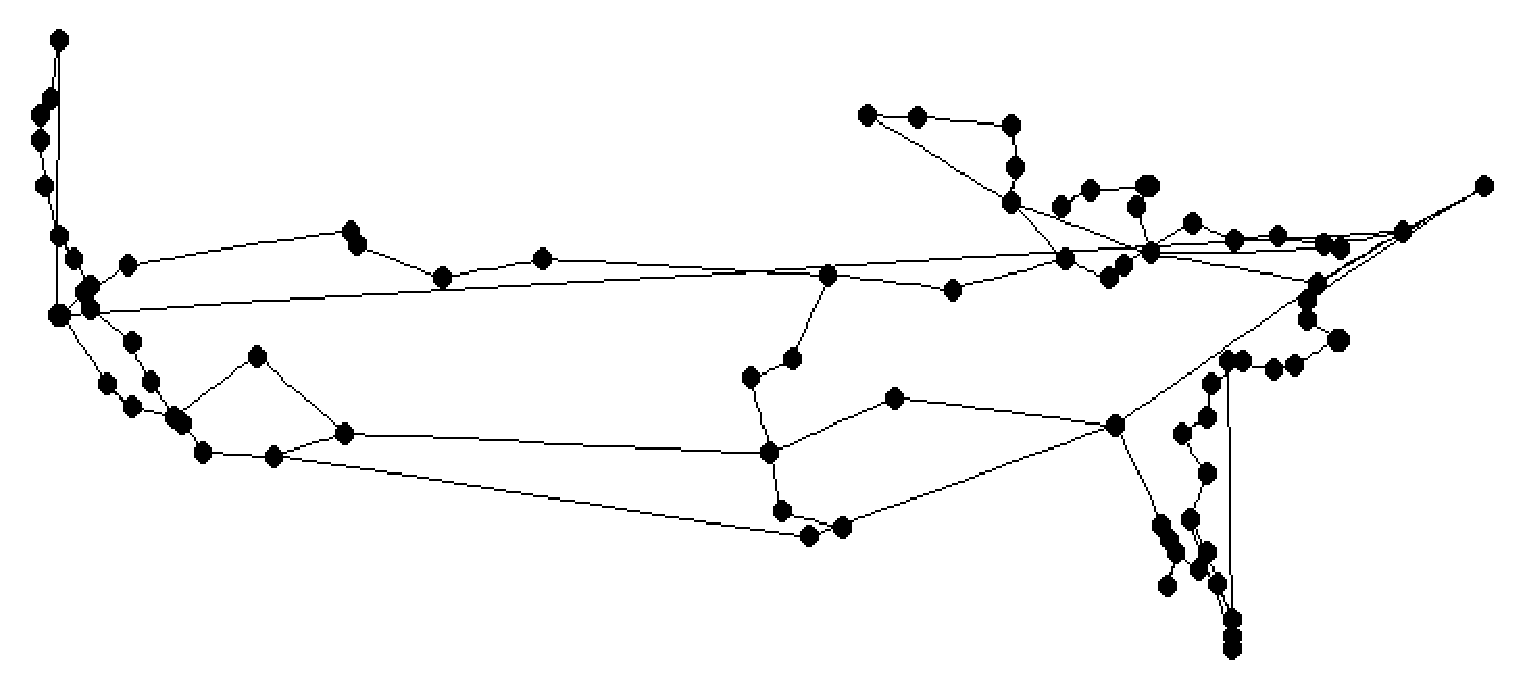
\includegraphics[scale=0.555]{data/AGIS.eps}
  \vspace{0mm}
  \caption{AGISのネットワークトポロジ}
  \label{fig:AGIS}
\end{figure}

\bigskip

\begin{figure}[htbp]
  \centering
  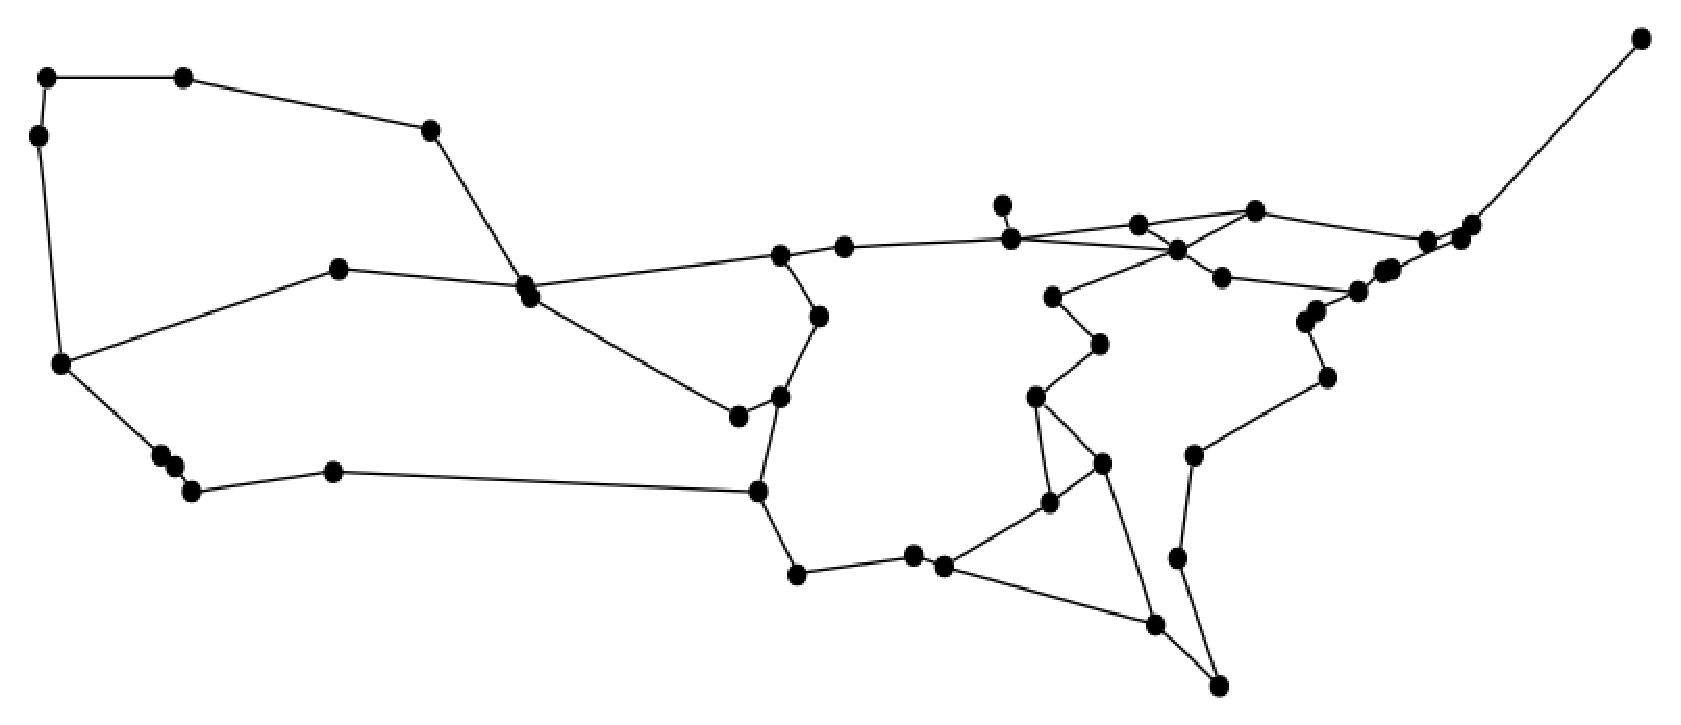
\includegraphics[scale=0.526]{data/At_Home_Network.eps}
  \vspace{0mm}
  \caption{At Home Networkのネットワークトポロジ}
  \label{fig:At}
\end{figure}

\begin{figure}[htbp]
  \centering
  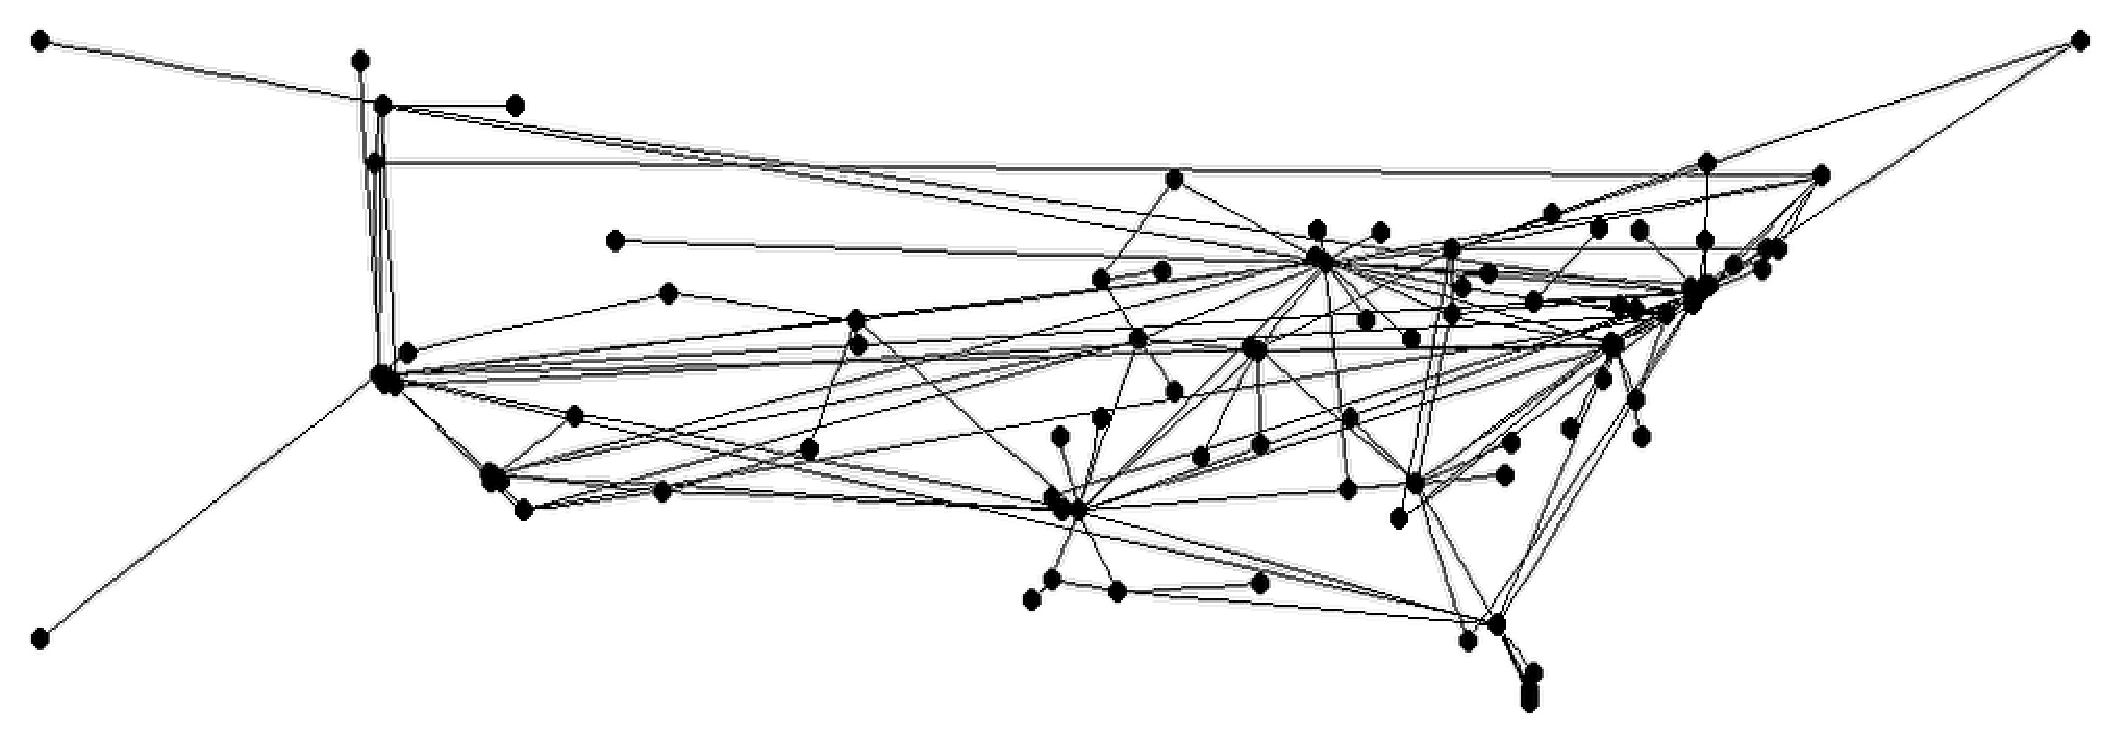
\includegraphics[scale=0.415]{data/ATT.eps}
  \vspace{0mm}
  \caption{ATTのネットワークトポロジ}
  \label{fig:ATT}
\end{figure}

\begin{figure}[htbp]
  \centering
  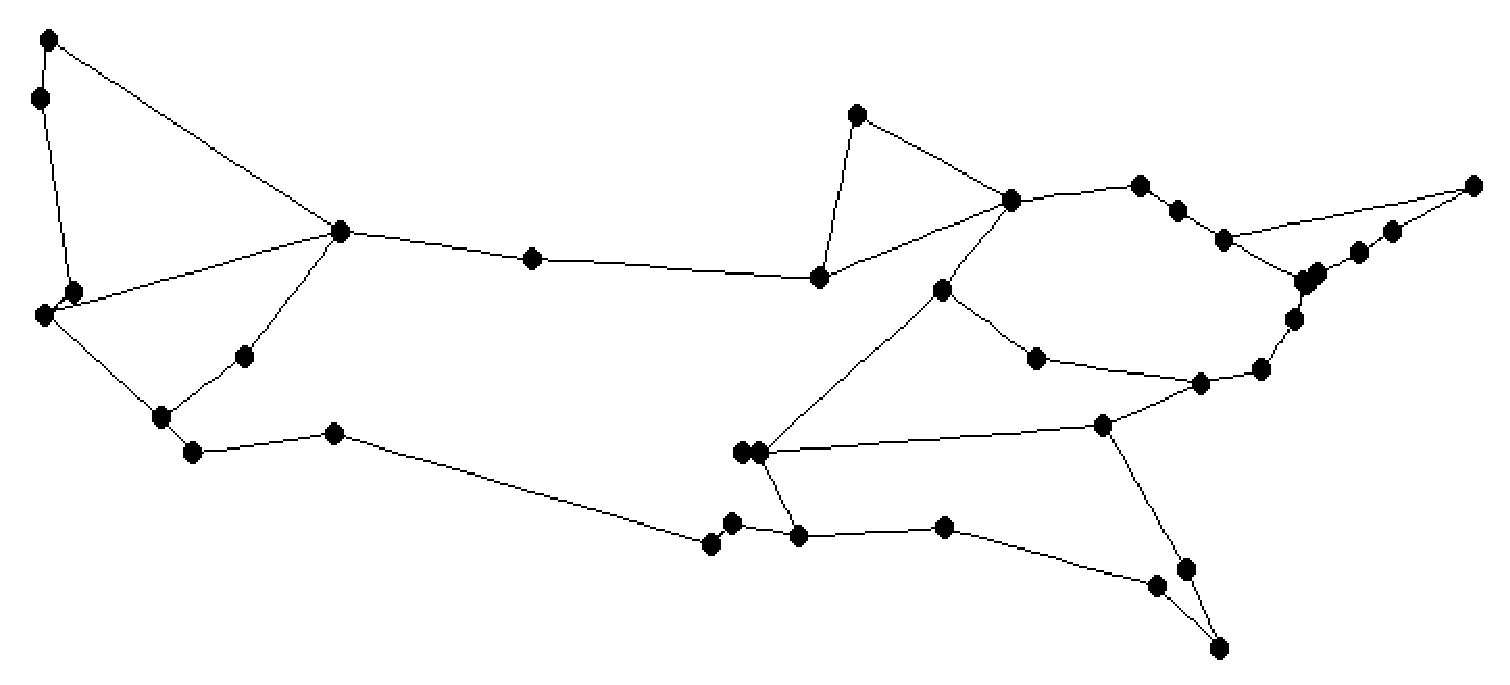
\includegraphics[scale=0.585]{data/CAIS_Internet.eps}
  \vspace{0mm}
  \caption{CAIS Internetのネットワークトポロジ}
  \label{fig:CAIS}
\end{figure}

\section{最適配置問題の定式化}
TS付与処理を行うルータの最適配置問題をP-メディアン問題及びP-センター問題を利用することで解決する.


\subsection{P-メディアン問題}
P-メディアン問題は,施設配置問題に関する最適化問題の一種である.
この問題では,ユーザから都市や施設などの位置において,
指定された数(p個)の施設を選択し,
それぞれのユーザと施設の重み付き距離の総距離を最小化することを目指すものである.
以下の式は今回の最適化問題を解決するにあたって,定式化した目的関数である.
尚,NodeはそれぞれのISPにおけるノードの総数,
$x_{i}$をノードiに施設を配置するかどうかを表す変数,
distanceをノードiからノードjまでの距離,
populationをユーザが通信の際にノードを使用していると考えられる人口である.

\begin{align}
  \label{p-median}
  \mbox{minimize}    \sum_{i \in \mbox{ Node }}\left(\mbox { population }_i \cdot \sum_{j \in \mbox { Node }, i \neq j}\left(\mbox { distance }_{i j} \cdot x_{i}\right)\right)
\end{align}

\begin{align}
  \text{subject to} \quad & \mbox{ Node }=\{A, B, C, D, E, F\dots\}                              \\
                          & x_{i}, i \in \mbox { Node }                                          \\
                          & \mbox { distance }_{i j}, i \in \mbox { Node }, j \in \mbox { Node } \\
                          & \mbox { population }_i, i \in \mbox { Node }
\end{align}


\subsection{P-センター問題}
P-センター問題は,施設配置問題に関する最適化問題の一種である.
この問題では,ユーザから都市や施設などの位置において,
指定された数(p個)の施設を選択し,
それぞれのユーザとP4スイッチの重み付き距離が極端に離れた組み合わせを作らないように配置することを目指すものである.
以下の式は今回の最適化問題を解決するにあたって,定式化した目的関数である.
尚,$v$を重み付き距離の最大距離を表す変数とする.
\begin{equation}
  \mbox{minimize} \quad v
\end{equation}

\begin{equation}
  \text{subject to} \quad v \geq \mbox{population}_i \cdot \mbox { distance }_{i j} \cdot x_{i}
\end{equation}

$$
  \mbox{および(6.2), (6.3), (6.4),(6.5)を満たす}
$$


\chapter{まとめ}
本論では,P4スイッチを用いてTS付与処理を行うノードをネットワークに設けることによって,先着販売システムを用いたオンラインチケット販売におけるユーザの公平性を担保する提案手法を示した.
性能評価において,提案方式の処理時間は送信処理のみ行うものと比較して,マイクロ秒以下であることが確認でき,提案方式の有効性を示した.
また上記のノードの最適配置問題をP-メディアン問題及びP-センター問題と捉え,定式化することによって,提案方式の改善方法を示した.
P-メディアン問題及びP-センター問題の最適化問題はNP困難であることが知られているため,遺伝的アルゴリズムなど各種手法を用いて解決することを検討する.

\chapterA{謝辞}
本研究を行うに当たり,ご指導を頂いた上山教授に感謝します.また日常,有益な議論
をして頂いた研究室の皆様に感謝します.

\begin{thebibliography}{99}
  \footnotesize
  \baselineskip 3.1mm
  \bibitem{P4}

  \,Pat Bosshart, et al.,
  P4: Programming Protocol-Independent Packet Processors, ACM SIGCOMM CCR, Vol. 44, No. 3, July 2014

  \bibitem{P4STA}
  \,R. Kundel, F. Siegmund, J. Blendin, A. Rizk and B. Koldehofe, "P4STA: High Performance Packet Timestamping with Programmable Packet Processors," NOMS 2020 - 2020 IEEE/IFIP Network Operations and Management Symposium, Budapest, Hungary, 2020, pp. 1-9, doi: 10.1109/NOMS47738.2020.9110290.

  \bibitem{LOBIN}
  X. Hong, C. Zheng, S. Zohren and N. Zilberman, "LOBIN: In-Network Machine Learning for Limit Order Books," 2023 IEEE 24th International Conference on High Performance Switching and Routing (HPSR), Albuquerque, NM, USA, 2023, pp. 159-166, doi: 10.1109/HPSR57248.2023.10147958.

  \bibitem{Clock Synchronization}
  Tomáš Martínek (CESNET), Mauro Campanella (GARR), Federico Pederzolli (FBK), Joseph Hill(UvA), Marinos Dimolianis (NTUA), Damian Parniewicz (PSNC), \\"White Paper:Timestamping and Clock Synchronisation in P4-Programmable Platforms", Document ID: GN4-3-22-49EC10
\end{thebibliography}

\chapterA{学会発表リスト}
\begin{quote}
  \begin{itemize}
    \item
          羽田秀平, 上山憲昭, “タイムスタンプを用いた公平なオンラインチケット販売方式”, 電子情報通信学会 2025 年総合大会, B-6, 東京, 2025年3月
  \end{itemize}
\end{quote}

\end{document}




%--------------------------------------------------
%<@dumy>
%下記の2行は、画像取り込み/引用のサンプル
%卒論作成のためには下記の2行の先頭に「%」を追加してコメントアウトすること。
%ただし、引用が0個の場合はエラーになるので、
%本文で引用を一つ以上行った後にコメントアウトすること。
%--------------------------------------------------
%\chapter{Dumyの章}

%--------------------------------------------------
%<@>
%文献挿入箇所
%--------------------------------------------------
%\bibliographystyle{unsrt}
%\bibliographyA{bib}
%--------------------------------------------------
\end{document}
%--------------------------------------------------
%<@>
%--------------------------------------------------


